\chapter{Testing}
\section*{Languages and Frameworks}
In order to test our system, we need to use a tool to create a \textit{virtual network} inside our machine; 
we used \texttt{mininet}\footnote{http://mininet.org/}, 
exploiting the \texttt{python2} APIs. To simulate input from an external application we also used a python2 library, called \texttt{requests}\footnote{https://docs.python-requests.org/en/latest/},
which is able to act like an HTTP client.\
Given that our developement environment is inside a virtual machine, we will keep the number of virtual devices relatively small, in order to not
overload the VM resources.

\section*{Scenario}
We want to simumlate a tipical data center scenario with a single LAN, implemented in a \textit{Spine-Leaf} topology. This configuration
is widely used thanks to it's easy scalability and sufficent redundancy.
\begin{figure}[h]
    \centering
    \caption{example of \textit{spine-leaf} topology}
    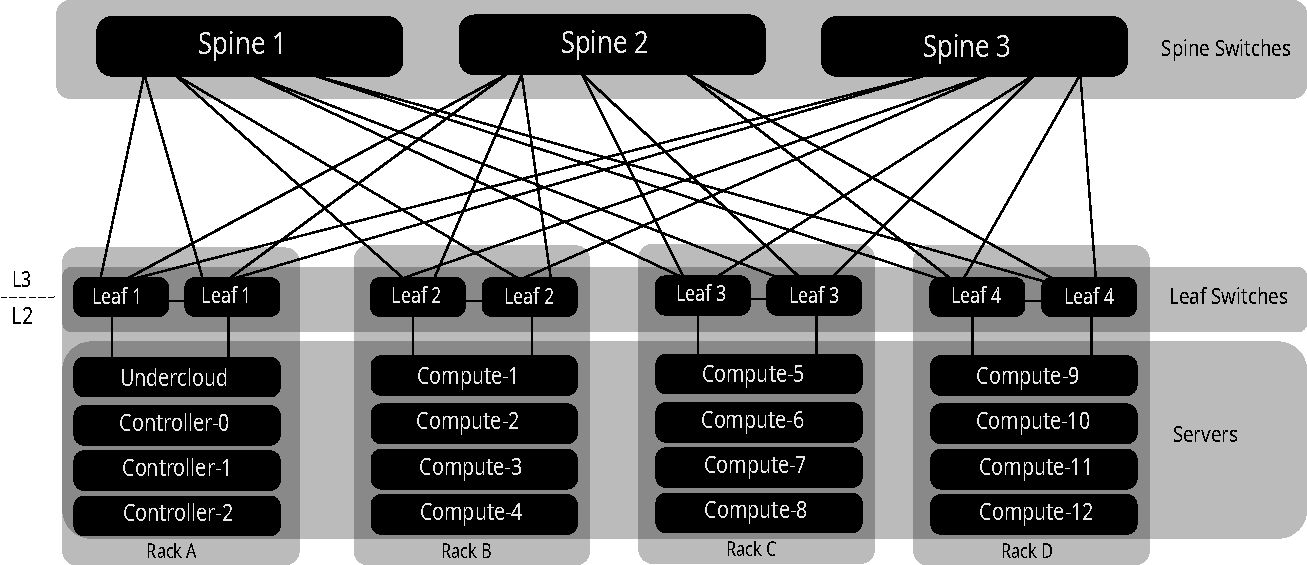
\includegraphics[width=0.90\textwidth]{img/spine_leaf.pdf}
\end{figure}

Using \texttt{mininet}, we can also simulate an episode of link failure, in order to test the system behaviour in this specific case. The system is able to
recompute a functional path between two host and use it to forward packets.
\newpage
\section{Ping Latency}
In order to mesure the network performance we will consider a fixed scenario with 2 spines, 3 leafs and 4 hosts for each leafs (i.e. 12 hosts in total);
for every host:
\begin{itemize}
    \item  we establish an intent with another randome chosed one;
    \item  we start a ping session, measuring the \texttt{round trip time} of each packet
    \item  the session end when 10 ping are succesfully exchanged, or the last timeout elapse
\end{itemize} 
\begin{figure}[h]
    \centering
    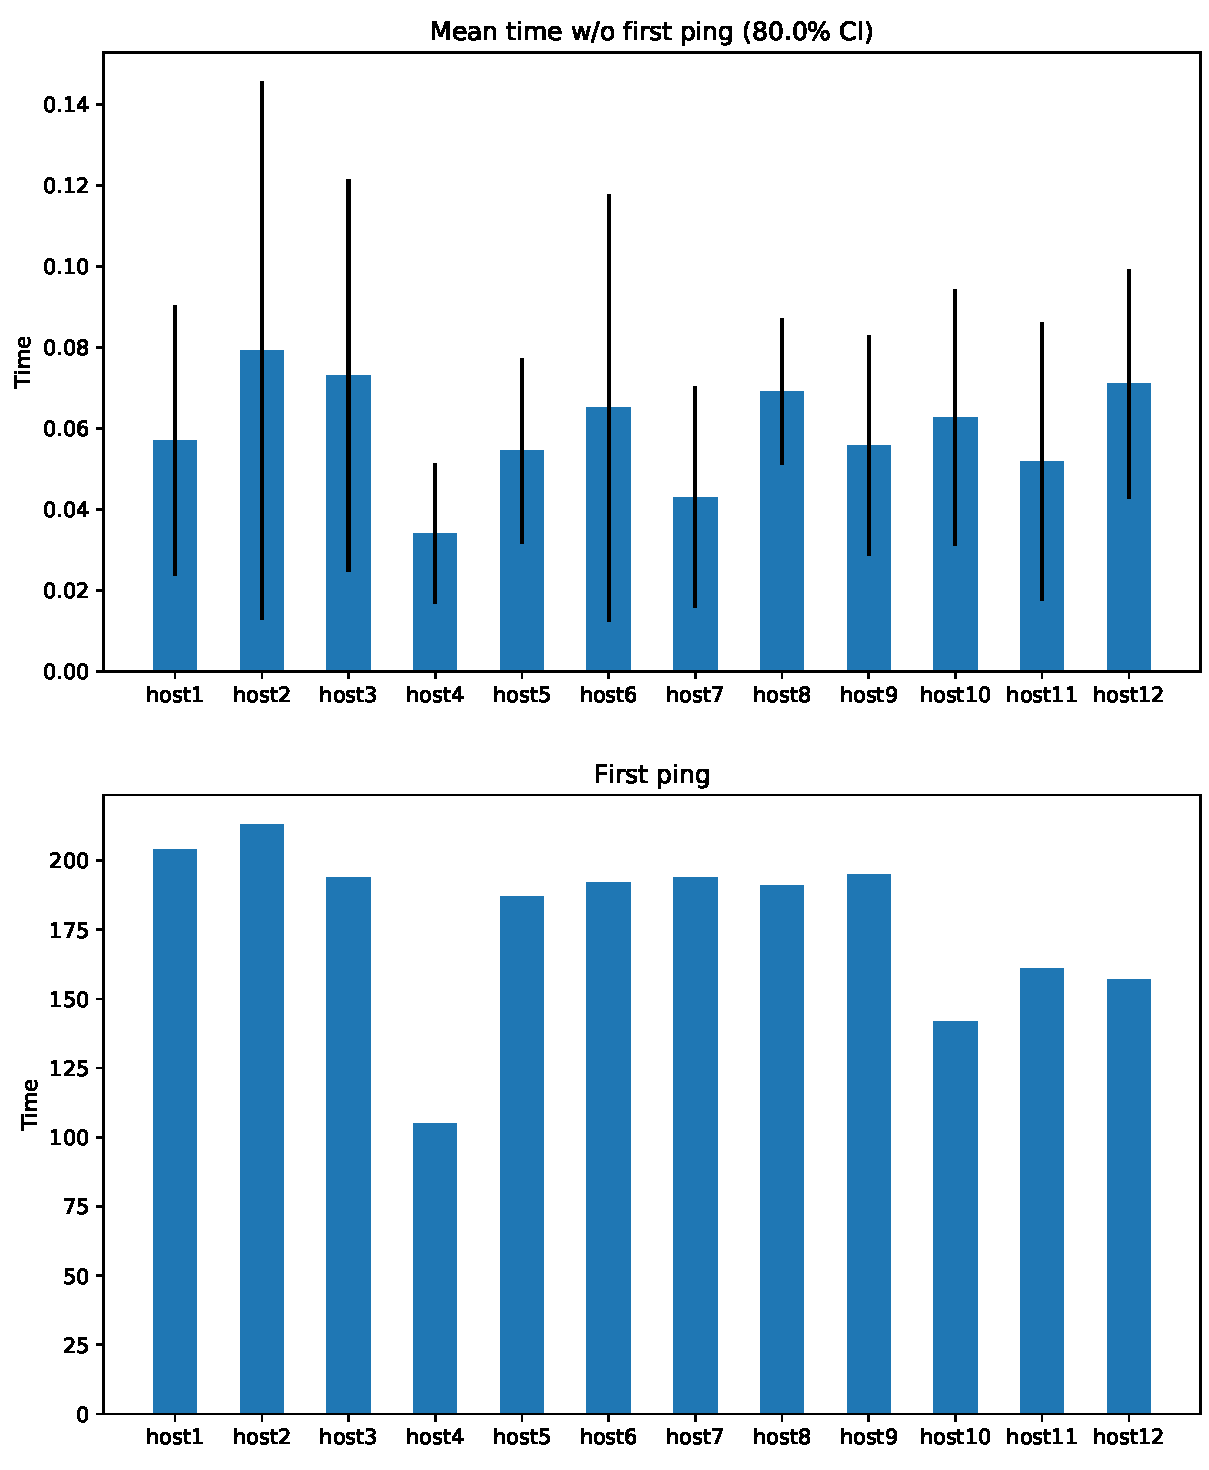
\includegraphics[width=.92\textwidth]{img/mean_ping_time.pdf}
    \caption{ping times with 12 hosts}
\end{figure}
First of all we motitor the number of \texttt{DESTINATION HOST UNREACHABLE} and \texttt{DUPLICATE}; those 2 parameters are at 0, confirming the correct
behaviourof the network.
The performance results are consistent with our expectation:
\begin{itemize}
    \item the first ping is significantly slower than the others, because it's processed by the controller, triggering the route establishment;
    \item subsequent pings are very fast (<1 ms), because they don't have to traverse "real" network cables.
\end{itemize}
\newpage
\begin{figure}[h]
    \centering
    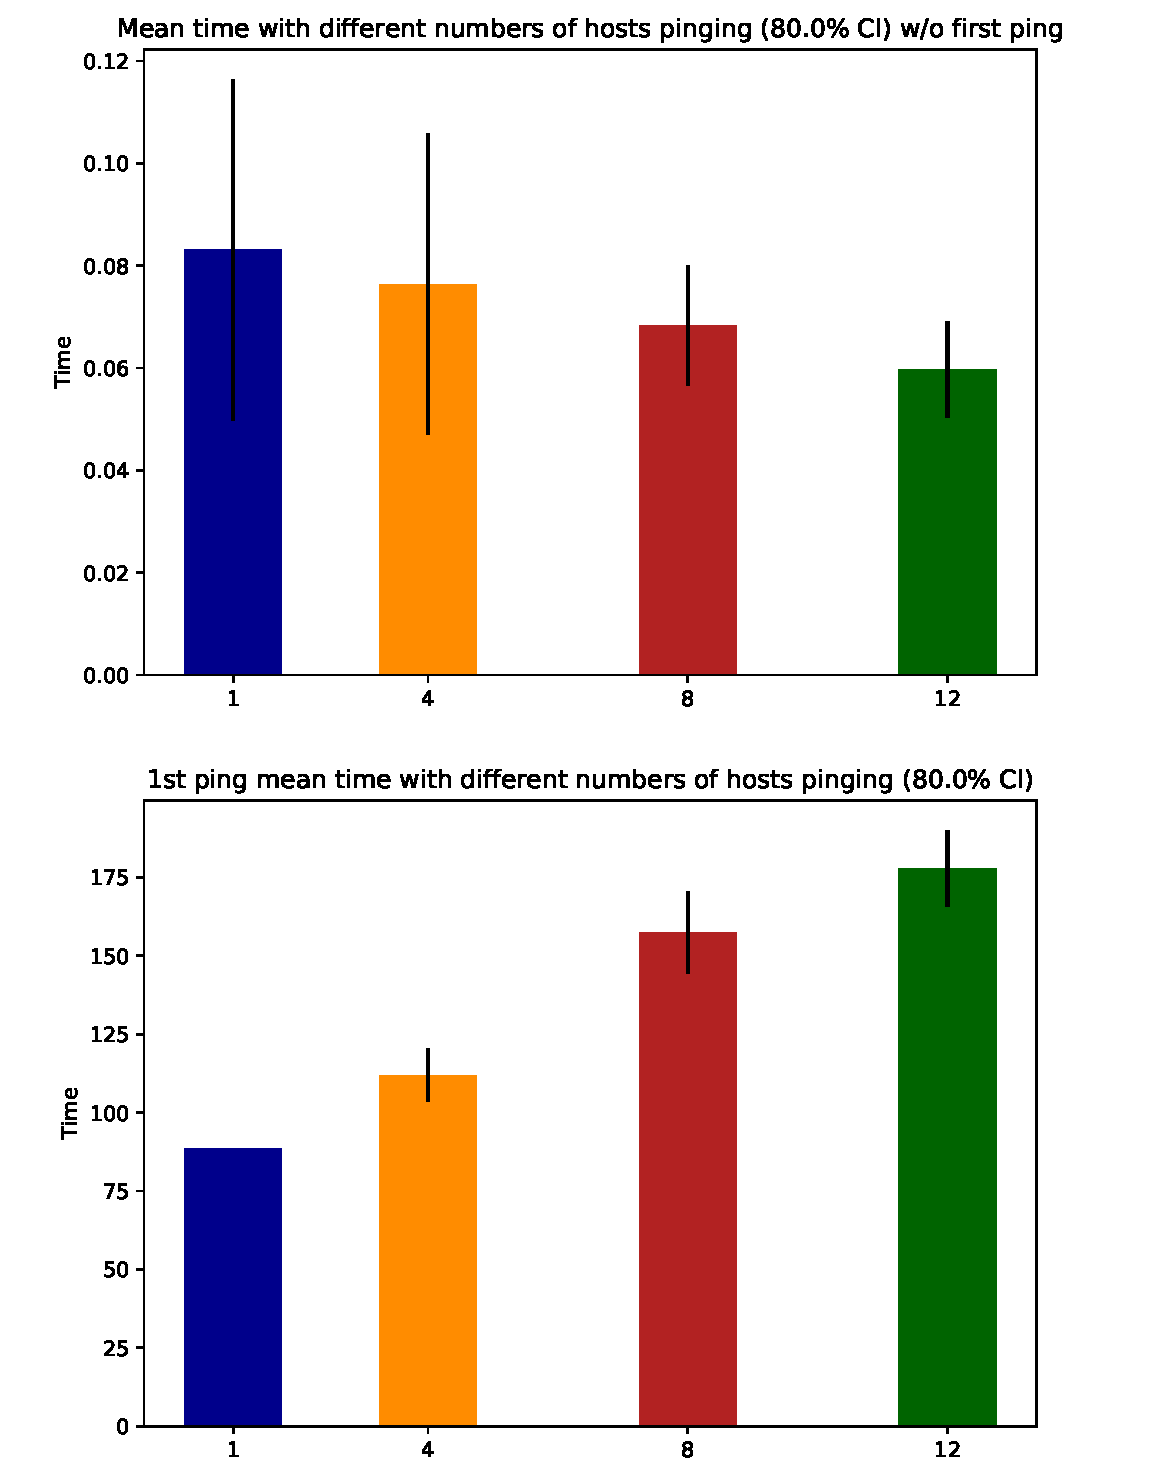
\includegraphics[width=.94\textwidth]{img/increasing_ping_time.pdf}
    \caption{ping times with differents loads}
\end{figure}
\noindent We also tried to evaluate the elasticity of the network with increasing load of traffic (i.e. increasing number of host pinging at the same time).\\
The time needed fot the first ping to complete tends to increase with the amount of traffic meanwhile the time for the others pings reamains preatty stable
(mind the confidence intervals). This is expected because route establishemnt is done by the controller in a centralized way (the requests will queue up);
once the route is establihed, switches will handle the traffic in a distributed manner, leading to optimal forwarding of traffic.